\question*{
    Simple Serve-and-Volley
}

\begin{arabicparts}
    \questionpart The state machine is

    \begin{figure}[ht]
        \centering
        \begin{tikzpicture}[->,>=stealth',shorten >=1pt,auto,node distance=5.5cm,
            scale = 1,transform shape]
        
        \node[state,initial] (Waiting) {$Waiting$};
        \node[state] (Passing) [below of=Waiting] {$Passing$};
        \node[state] (Checking) [right of=Passing] {$Checking $};
        \node[state,accepting] (Victory) [above of=Checking] {$Victory$};
        
        \path (Waiting) edge              node {$L$} (Passing)
                (Passing) edge              node {$Time$} (Checking)
                (Checking) edge[bend left]              node[left] {$L ,\; ballPos = 0$} (Victory)
                (Checking) edge[bend right]              node[right] {$R ,\; ballPos = n-1$} (Victory)
                (Victory) edge              node {$Time$} (Waiting);
        
        \end{tikzpicture}
        \caption{State Machine for the game.}
        \label{fig:statemach}
    \end{figure}
    
    The switches were connected, see \autoref{fig:connected}. The
    following code was used for the interrupts:

    \begin{lstlisting}[language=C++]
// <-- Indicates a skip in code
volatile bool leftHit = false, rightHit = false;
//
volatile uint16_t timeLeftHit = 0, timeRightHit = 0;
// 

void setup(){
    //
    pinMode(leftPlayer, INPUT);
    attachInterrupt(digitalPinToInterrupt(leftPlayer), leftPlayerHit, FALLING);
    pinMode(rightPlayer, INPUT);
    attachInterrupt(digitalPinToInterrupt(rightPlayer), rightPlayerHit, FALLING);
}

// 

void leftPlayerHit(){
  leftHit = true;
  timeLeftHit = 0;
  return;
}

void rightPlayerHit(){
  rightHit = true;
  timeRightHit = 0;
  return;
}
    \end{lstlisting}
    
    \begin{figure}[ht]
        \centering
        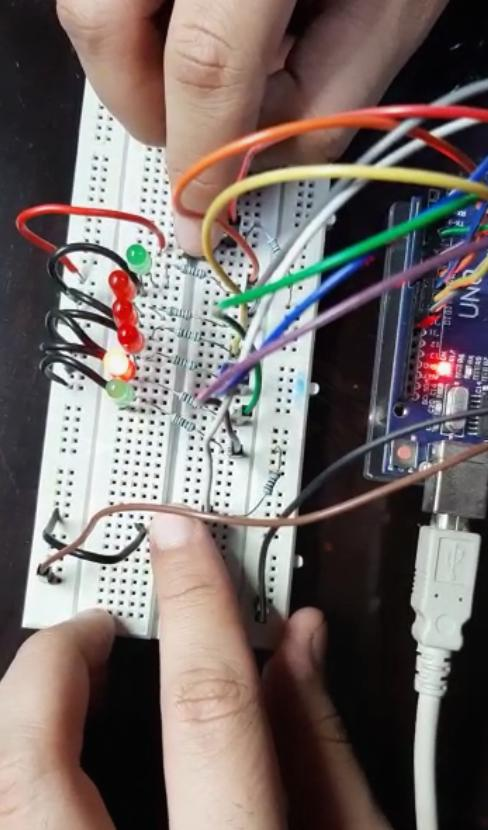
\includegraphics[width=0.6\textwidth, angle=90]{fig/arduinoconnected-min.jpg}
        \caption{Connected setup}
        \label{fig:connected}
    \end{figure}

    \questionpart The LEDs were connected as in \autoref{fig:connected}. One of
    my red LEDs seems to not light up, so it looks a bit awkward in the
    demonstration. The following code is used for the light propagation:

    \begin{lstlisting}[language=C++]
// <-- Indicates a skip in code
// LED outputs
int redPin[4] = {5, 9, 10, 11}; // pins for red LEDs, from the left

//
uint8_t ball[2] = {0, 1}; // position 0, moving right
//
void loop(){
    //

    switch (state)
    {
    //

    case 1:
      // game in play
      delay(600); // delay to control clock speed
      if(ball[0] != 0 && ball[0] != 3){
        // somewhere in the middle
        ball[0] += ball[1]; // x = x + v.dt
        changeOutputs();
        break;
      }
      else{
        ballInRange = (ball[0] == 0) ? 1 : -1;
        state = (ball[0] == 0) ? 2 : 3;
        // start counter
        ballWaitStart = millis();
      }
      break;
    
   //
}

//

void changeOutputs(){
    for(int i = 0; i < 4; i++){
        if(ball[0] == i){
            analogWrite(redPin[i], 255);
        }
        else{
            analogWrite(redPin[i], 0);
        }
    }
}
    \end{lstlisting}

    \questionpart The setup was completed, and a video demonstration may be
    found in this
    \href{https://drive.google.com/drive/folders/1oetbbPwgUUYHVBNe5_pIktCHrrqsNl7a?usp=sharing}{
        Google Drive Folder}.

\end{arabicparts}